\chapter{Definitions and datasets\label{chap::def}}

\begin{marginfigure}%
	% 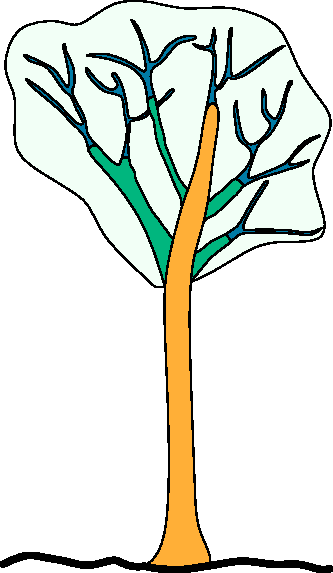
\includegraphics[width=\marginparwidth]{./Figures/ign_tree.pdf}
	\begin{tikzpicture}
	\node (tree) at (0, 0) {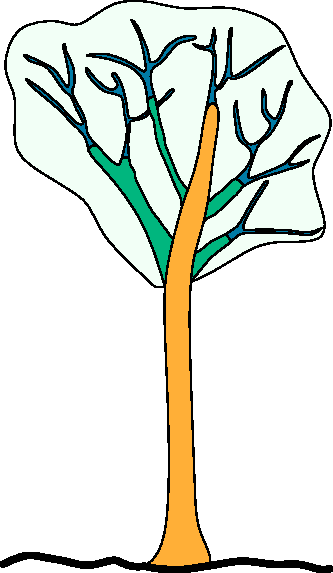
\includegraphics[width=\marginparwidth]{./Figures/ign_tree.pdf}};
	\matrix[below = -0.2cm of tree] {
		\node [draw, shape = rectangle, fill = egyptYellow, label = right:Bole] {}; \\
		\node [draw, shape = rectangle, fill = egyptGreen, label = right:Large branches] {}; \\
		\node [draw, shape = rectangle, fill = egyptBlue, label = right:Small branches] {}; \\
	};
\end{tikzpicture}
	\caption{Scheme of tree components.\label{fig::ign_tree}}
\end{marginfigure}

This volume is distributed among three parts:
\begin{description}
	\item[Bole]: The main stem, starting from the base and up to a diameter of \SI{7}{\centi\metre}
	\item[Large branches]: Branches up to a diameter of \SI{7}{\centi\metre}
	\item[Small branches]: Branches from a diameter of \SI{7}{\centi\metre} to \SI{0}{\centi\metre}
\end{description}



% \begin{figure*}[h]
% 	\begin{tikzpicture}
	%% Level 0
	\node (orig) at (0, 0) {Whole tree};
	
	%% Level 1
	\node[below right = of orig] (belowground) {Below-ground};
	\node[above right = of orig] (aboveground) {Above-ground};
	
	%% Level 2
	\node[above right = of aboveground] (stem) {Main stem};
	\node[right = of aboveground] (lat) {Lateral};
	\node[below right = of aboveground] (fol) {Foliage};
	
	\node[right = of belowground] (root) {Root};

	%% Level 3
	\node[above right = of stem] (stemtop) {Stem top};
	\node[right = of stem] (bole) {Bole};
	\node[below right = of stem] (stump) {Stump};

	\node[below right = of lat] (lbranch) {Large branches};
	\node[above right = of lat] (sbranch) {Small branches};

	\begin{scope}[on background layer] % From background library
		% \fill[lightGrey] (2.735294,0) rectangle (6,6);
		\node[fit=(belowground)(aboveground), fill = lightGrey, inner sep=5mm] {};
	\end{scope}

\end{tikzpicture}
% 	\caption{Flowchart.\label{fig::flowchart}}
% \end{figure*}
